\newpage

\section{Feedback Control with a Servo and Accelerometer}

\subsection{Parts List}

\begin{enumerate}[itemsep=-5pt]
\item CPX/CPB
\item USB Cable
\item Laptop
\item servo
\item Alligator clips (x3)
\end{enumerate}

\subsection{Learning Objectives}
\begin{enumerate}[itemsep=-5pt]
\item Understand how to compute roll and pitch from an accelerometer
\item Learn the fundamental concepts of feedback control
\item Learn how to Combine two codes (servo code and accelerometer code into one)
\end{enumerate}

\subsection{Getting Started}

Feedback control can be its own course or multiple courses but can be broken down into a few simple steps. The goal of feedback control is to drive the “state” of a “system” to a desired “command” by sending a “control” signal to the “system”. I explain this in much more detail in a \href{https://www.youtube.com/watch?v=PAK5V8wzVXY&list=PL_D7_GvGz-v30U58EUUOdJGgO4u75DXoB&index=1}{controls overview Youtube video}. For this lab we are going to make the bare bones circuitry required for pitch angle control of an airplane. The “system” then is the aircraft. The “state” is the “pitch” angle (measured by the CPX), the “command” is the desired pitch angle (programmed by you the pilot in command) and the “control” signal is the elevator command (actuated by a servo). I’m using the same circuit I created in the other servo projects (See chapter \ref{s:pwm}). Here’s the circuit for simple reference. Remember the servo has 3 pins - the brown or black wire is GND, the red wire needs to go to a 5V signal so for the CPX it needs to go to the VOUT pin and the yellow or white wire is the signal wire which need to go to an analog port on the CPX that supports PWM signals.
\begin{figure}[H]
  \begin{center}
    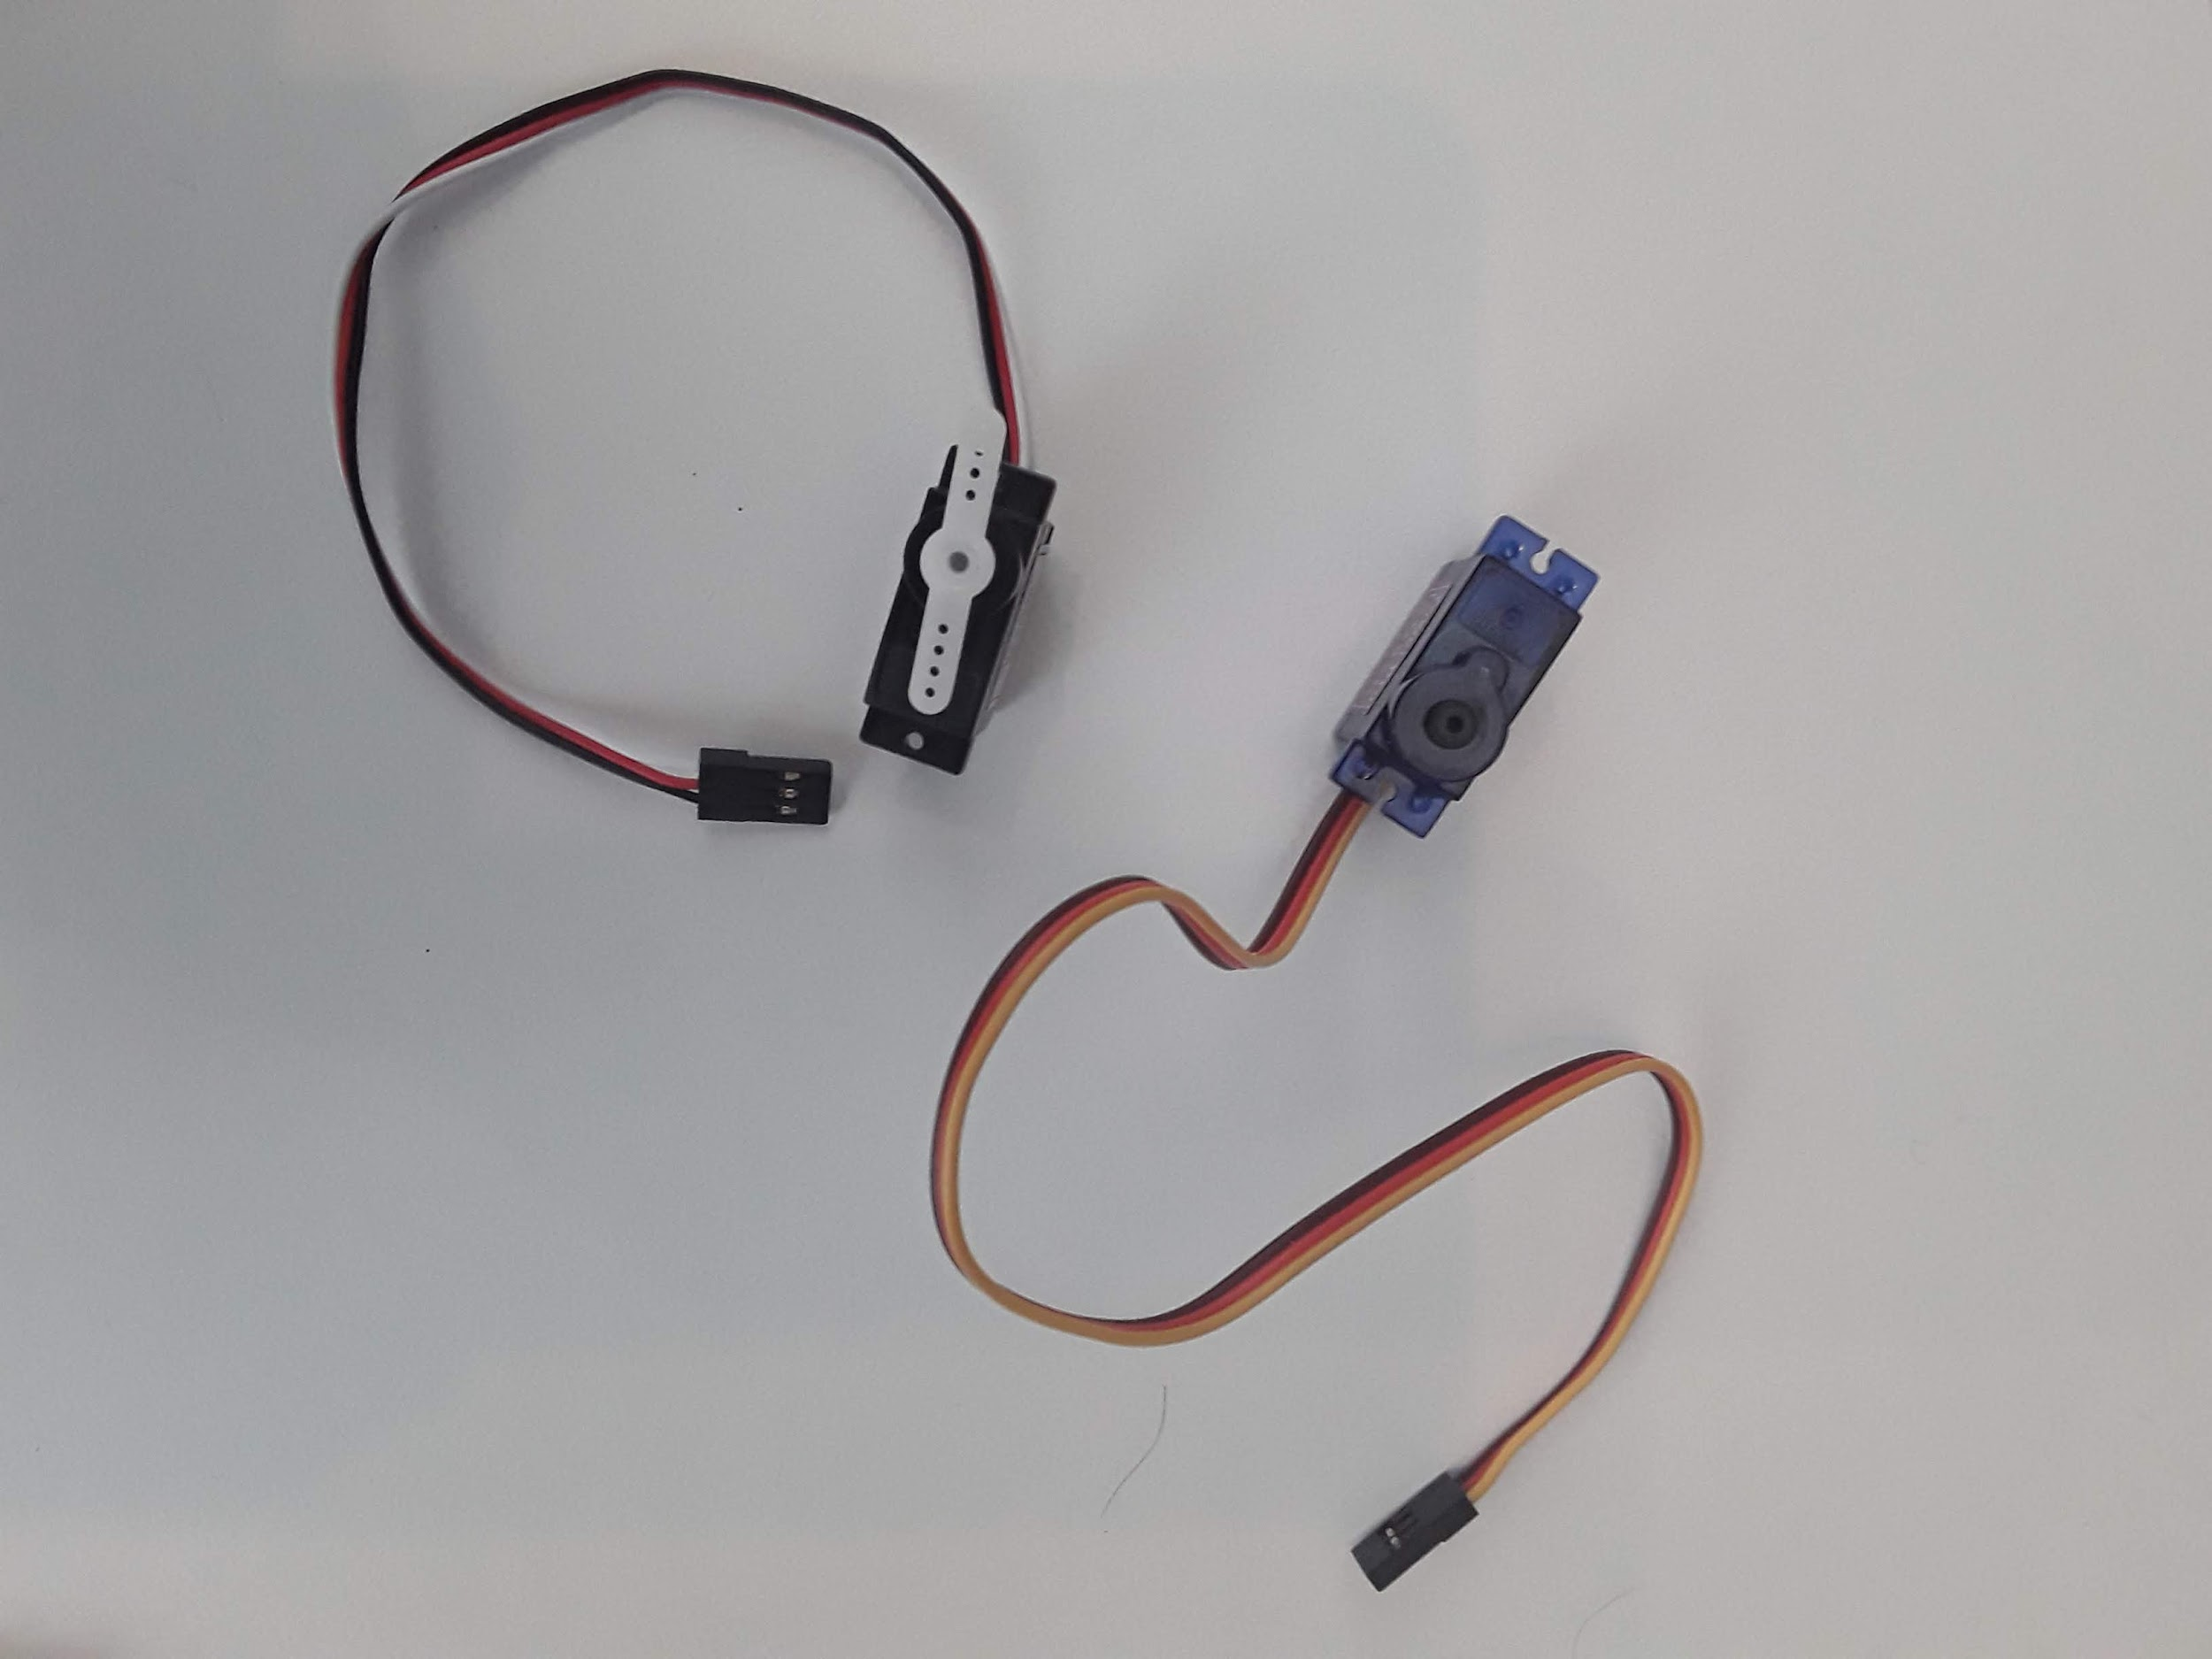
\includegraphics[width=0.8\textwidth]{Figures/servo.jpeg}
  \end{center}
\end{figure}
The elevator on an airplane is a control surface responsible for pitching the aircraft up and down. For this example we are going to assume that the desired pitch angle is 0. This means our “error” signal is going to be 0 minus the pitch angle. Our “control” signal will be the angle of the elevator. As I said, we are going to use a servo to control the elevator so this just means we need a way to relate our “error” signal to servo pulse width. There are a few steps here before we can move on. First, we need to relate our “error” signal to the “control” signal which will be the elevator pitch angle. I’ve made a table below to explain what I mean.
\begin{table}[H]
\begin{center}
\begin{tabular}{|c|c|c|}
\hline
Pitch (deg) & Error (deg) & Elevator (deg) \\
\hline
-90 & 90 & +90 \\
\hline
0 & 0 & -90 \\
\hline
+90 & -90 & -90 \\
\hline
\end{tabular}
\end{center}
\end{table}
This table basically says that if the aircraft is level with a pitch angle of zero I want the elevator to be zero as well. If the aircraft pitches down, I want the elevator to pitch up and counteract that rotation. Using these three data points I can create a simple equation to relate elevator angle to pitch angle.
\begin{equation}
\delta_e = -\theta
\end{equation}
Now that we have the elevator pitch angle we need to relate this to the servo angle. Servo can only move from 0 to 180 degrees which means we can’t have the servo go negative. Thus we need to offset the elevator angle to the servo angle. Again we can make a table here.
\begin{table}[H]
\begin{center}
\begin{tabular}{|c|c|}
\hline
Elevator (deg) & Servo (deg)\\
\hline
-90 & 0 \\
\hline
0 & 90 \\
\hline
+90 & 180 \\
\hline
\end{tabular}
\end{center}
\end{table}
This also results in a simple equation to relate servo angle to elevator angle.
\begin{equation}
s = \delta_e + 90
\end{equation}
Finally, we can then use our calibration coefficients (See chapter \ref{s:pwm}) to relate servo angle to pulse width. When I calibrated my servo I obtained the following equation where P is the pulse and s is the servo angle.
\begin{equation}
Pulse = 0.6 + 0.01*Angle
\end{equation}
With these 3 equations I can now program my servo to respond to changes in the pitch angle of the CPX. I did forget one minor detail and that is measuring the pitch angle itself. This is similar to measuring the angle of a pendulum (See chapter \ref{s:pendulum}). I’m going to rotate the CPX in the X/Z plane which can be done by rotating the USB cable where it plugs into the CPX. In this case we can ignore the Y axis data. If you print the raw accelerometer data, you’ll notice that when you place the CPX directly onto a flat surface, the x and y axes read a value around 0, while the z axis reads around gravity. If you then rotate the sensor clockwise 90 degrees, the x axis is reading about gravity while the z axis is now zero. This means we can form a triangle and get the angle using these two axes using the equation below which gives angle in degrees.
\begin{equation}
\theta = tan^{-1}(x/y)\frac{180}{\pi}
\end{equation}
On the CPX specifically we want to import the math module and use the atan2 function. With this equation I can finally put it all together. Here is my code which again is also \href{https://github.com/cmontalvo251/Microcontrollers/blob/master/Circuit_Playground/CircuitPython/Servo/feedback_control_servo.py}{online on Github}.
\begin{figure}[H]
  \begin{center}
    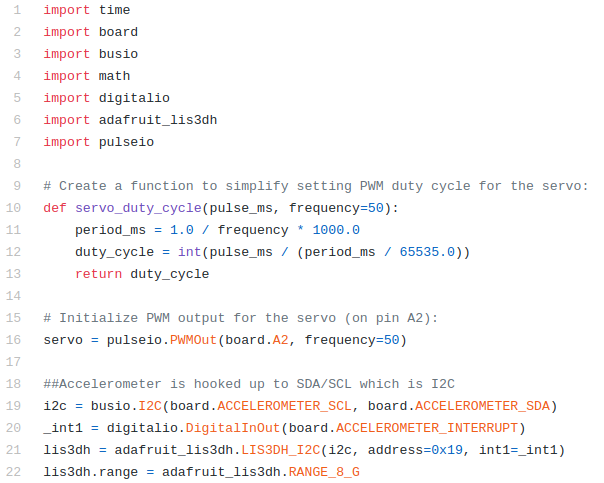
\includegraphics[width=0.8\textwidth]{Figures/feedback1.png}
  \end{center}
\end{figure}
The first 22 lines here will hopefully seem familiar. Line 1-7 are import commands of all the various modules needed. Lines 10-13 create the definition that converts pulse width to duty cycle. Line 16 creates the servo and lines 19-22 create the accelerometer. Hopefully this is a good example of combining different codes together to get a more complex piece of software. Lines 24-45 include a very long while loop. I will try and go through each line. Line 26 grabs the accelerometer data on the CPX. Line 28 uses the x and z axis accelerometer data and converts the values to pitch angle using the atan2 function in the math module which was imported on line 4. Line 30 computes the elevator pitch angle and line 32 computes the servo deflection angle. Line 34-37 is a type of signal conditioner called a saturation filter. Basically, I don’t want the servo to break because I tried to make the servo rotate more than 180 degrees or less than 0 degrees. So I created two if statements that restrict the servo to be within these two values. If the servo angle is less than 0 as stated on line 34, the servo angle is set to 0 on line 35. If the servo angle is greater than 180 as stated in line 36 the servo angle is set to 180.
\begin{figure}[H]
  \begin{center}
    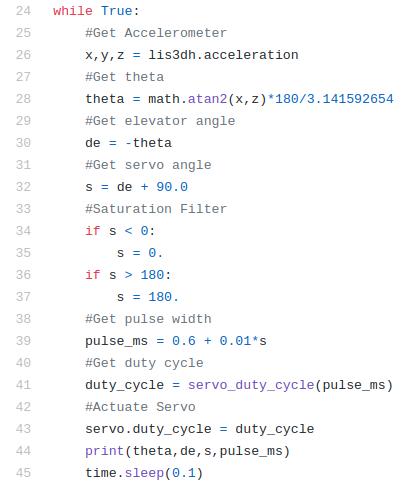
\includegraphics[width=0.6\textwidth]{Figures/feedback2.png}
  \end{center}
\end{figure}
Line 39 uses the calibration equation from the previous experiment to convert servo angle to pulse width. You’ll need to replace these numbers with your servo since all servos are different. Line 41 uses the definition created on lines 10-13 to convert pulse width to duty cycle. Line 43 makes the servo move. Line 44 prints everything to Serial for debugging purposes and line 45 pauses the script for 0.1 seconds which helps with some twitchiness in the servo. When I did this I didn’t have to program a complementary filter so I guess the servo may have it’s own low pass filter. Either way this circuit is ready to be placed on an aircraft. Whether or not it is effective is a completely different story. I’ll leave that discussion to your controls professor. Note you can also include the angular rate sensor and use that as derivative gain as well.

\subsection{Assignment}

Upload a PDF with all of the photos and text below included. My recommendation is for you to create a Word document and insert all the photos and text into the document. Then export the Word document to a PDF. For videos I suggest uploading the videos to Google Drive, turn on link sharing and include a link in your PDF.

\begin{enumerate}[itemsep=-5pt]
\item Explain your circuit and what wires go where - 10\%
\item Explain your code. Specifically discuss any changes you have to make from my code to get it to work on your circuit. At a minimum you will need to change line 39. What I mean by that is that I want you to use your linear regression model from a previous lab so that it better controls the angle of your servo. You may also have to change the saturation filter. - 20\%
\item Show your servo moving as you rotate the CPX. Rotate the CPX positive and verify that the servo moves negative. - 50\%
\item Verify that your saturation filter works correctly by rotating your CPX past 90 degrees - 20\% \item Again make sure that your face is in the video at some point and you introduce yourself.
\end{enumerate}